\documentclass[]{article}
\usepackage{lmodern}
\usepackage{amssymb,amsmath}
\usepackage{ifxetex,ifluatex}
\usepackage{fixltx2e} % provides \textsubscript
\ifnum 0\ifxetex 1\fi\ifluatex 1\fi=0 % if pdftex
  \usepackage[T1]{fontenc}
  \usepackage[utf8]{inputenc}
\else % if luatex or xelatex
  \ifxetex
    \usepackage{mathspec}
  \else
    \usepackage{fontspec}
  \fi
  \defaultfontfeatures{Ligatures=TeX,Scale=MatchLowercase}
\fi
% use upquote if available, for straight quotes in verbatim environments
\IfFileExists{upquote.sty}{\usepackage{upquote}}{}
% use microtype if available
\IfFileExists{microtype.sty}{%
\usepackage{microtype}
\UseMicrotypeSet[protrusion]{basicmath} % disable protrusion for tt fonts
}{}
\usepackage[margin=1in]{geometry}
\usepackage{hyperref}
\PassOptionsToPackage{usenames,dvipsnames}{color} % color is loaded by hyperref
\hypersetup{unicode=true,
            pdftitle={Module 2: Recommeded exercises},
            pdfauthor={Stefanie Muff, Department of Mathematical Sciences, NTNU},
            colorlinks=true,
            linkcolor=Maroon,
            citecolor=Blue,
            urlcolor=blue,
            breaklinks=true}
\urlstyle{same}  % don't use monospace font for urls
\usepackage{color}
\usepackage{fancyvrb}
\newcommand{\VerbBar}{|}
\newcommand{\VERB}{\Verb[commandchars=\\\{\}]}
\DefineVerbatimEnvironment{Highlighting}{Verbatim}{commandchars=\\\{\}}
% Add ',fontsize=\small' for more characters per line
\usepackage{framed}
\definecolor{shadecolor}{RGB}{248,248,248}
\newenvironment{Shaded}{\begin{snugshade}}{\end{snugshade}}
\newcommand{\KeywordTok}[1]{\textcolor[rgb]{0.13,0.29,0.53}{\textbf{#1}}}
\newcommand{\DataTypeTok}[1]{\textcolor[rgb]{0.13,0.29,0.53}{#1}}
\newcommand{\DecValTok}[1]{\textcolor[rgb]{0.00,0.00,0.81}{#1}}
\newcommand{\BaseNTok}[1]{\textcolor[rgb]{0.00,0.00,0.81}{#1}}
\newcommand{\FloatTok}[1]{\textcolor[rgb]{0.00,0.00,0.81}{#1}}
\newcommand{\ConstantTok}[1]{\textcolor[rgb]{0.00,0.00,0.00}{#1}}
\newcommand{\CharTok}[1]{\textcolor[rgb]{0.31,0.60,0.02}{#1}}
\newcommand{\SpecialCharTok}[1]{\textcolor[rgb]{0.00,0.00,0.00}{#1}}
\newcommand{\StringTok}[1]{\textcolor[rgb]{0.31,0.60,0.02}{#1}}
\newcommand{\VerbatimStringTok}[1]{\textcolor[rgb]{0.31,0.60,0.02}{#1}}
\newcommand{\SpecialStringTok}[1]{\textcolor[rgb]{0.31,0.60,0.02}{#1}}
\newcommand{\ImportTok}[1]{#1}
\newcommand{\CommentTok}[1]{\textcolor[rgb]{0.56,0.35,0.01}{\textit{#1}}}
\newcommand{\DocumentationTok}[1]{\textcolor[rgb]{0.56,0.35,0.01}{\textbf{\textit{#1}}}}
\newcommand{\AnnotationTok}[1]{\textcolor[rgb]{0.56,0.35,0.01}{\textbf{\textit{#1}}}}
\newcommand{\CommentVarTok}[1]{\textcolor[rgb]{0.56,0.35,0.01}{\textbf{\textit{#1}}}}
\newcommand{\OtherTok}[1]{\textcolor[rgb]{0.56,0.35,0.01}{#1}}
\newcommand{\FunctionTok}[1]{\textcolor[rgb]{0.00,0.00,0.00}{#1}}
\newcommand{\VariableTok}[1]{\textcolor[rgb]{0.00,0.00,0.00}{#1}}
\newcommand{\ControlFlowTok}[1]{\textcolor[rgb]{0.13,0.29,0.53}{\textbf{#1}}}
\newcommand{\OperatorTok}[1]{\textcolor[rgb]{0.81,0.36,0.00}{\textbf{#1}}}
\newcommand{\BuiltInTok}[1]{#1}
\newcommand{\ExtensionTok}[1]{#1}
\newcommand{\PreprocessorTok}[1]{\textcolor[rgb]{0.56,0.35,0.01}{\textit{#1}}}
\newcommand{\AttributeTok}[1]{\textcolor[rgb]{0.77,0.63,0.00}{#1}}
\newcommand{\RegionMarkerTok}[1]{#1}
\newcommand{\InformationTok}[1]{\textcolor[rgb]{0.56,0.35,0.01}{\textbf{\textit{#1}}}}
\newcommand{\WarningTok}[1]{\textcolor[rgb]{0.56,0.35,0.01}{\textbf{\textit{#1}}}}
\newcommand{\AlertTok}[1]{\textcolor[rgb]{0.94,0.16,0.16}{#1}}
\newcommand{\ErrorTok}[1]{\textcolor[rgb]{0.64,0.00,0.00}{\textbf{#1}}}
\newcommand{\NormalTok}[1]{#1}
\usepackage{graphicx,grffile}
\makeatletter
\def\maxwidth{\ifdim\Gin@nat@width>\linewidth\linewidth\else\Gin@nat@width\fi}
\def\maxheight{\ifdim\Gin@nat@height>\textheight\textheight\else\Gin@nat@height\fi}
\makeatother
% Scale images if necessary, so that they will not overflow the page
% margins by default, and it is still possible to overwrite the defaults
% using explicit options in \includegraphics[width, height, ...]{}
\setkeys{Gin}{width=\maxwidth,height=\maxheight,keepaspectratio}
\IfFileExists{parskip.sty}{%
\usepackage{parskip}
}{% else
\setlength{\parindent}{0pt}
\setlength{\parskip}{6pt plus 2pt minus 1pt}
}
\setlength{\emergencystretch}{3em}  % prevent overfull lines
\providecommand{\tightlist}{%
  \setlength{\itemsep}{0pt}\setlength{\parskip}{0pt}}
\setcounter{secnumdepth}{0}
% Redefines (sub)paragraphs to behave more like sections
\ifx\paragraph\undefined\else
\let\oldparagraph\paragraph
\renewcommand{\paragraph}[1]{\oldparagraph{#1}\mbox{}}
\fi
\ifx\subparagraph\undefined\else
\let\oldsubparagraph\subparagraph
\renewcommand{\subparagraph}[1]{\oldsubparagraph{#1}\mbox{}}
\fi

%%% Use protect on footnotes to avoid problems with footnotes in titles
\let\rmarkdownfootnote\footnote%
\def\footnote{\protect\rmarkdownfootnote}

%%% Change title format to be more compact
\usepackage{titling}

% Create subtitle command for use in maketitle
\providecommand{\subtitle}[1]{
  \posttitle{
    \begin{center}\large#1\end{center}
    }
}

\setlength{\droptitle}{-2em}

  \title{Module 2: Recommeded exercises}
    \pretitle{\vspace{\droptitle}\centering\huge}
  \posttitle{\par}
  \subtitle{TMA4268 Statistical Learning V2020}
  \author{Stefanie Muff, Department of Mathematical Sciences, NTNU}
    \preauthor{\centering\large\emph}
  \postauthor{\par}
      \predate{\centering\large\emph}
  \postdate{\par}
    \date{January xx and yy, 2020}

\usepackage{xcolor}

\begin{document}
\maketitle

{
\hypersetup{linkcolor=black}
\setcounter{tocdepth}{2}
\tableofcontents
}
\section{Plan for the introductory
lecture}\label{plan-for-the-introductory-lecture}

\textbf{First hour with all students:}

14.15: getting to know group members, connecting to the screen,
introduction\\
14.15-14.55: work with Problem 2 above, and if time look at Problem 1,
Exam 2018 Problem 2, and Problem 3.\\
14.55-15.00: summing up, discussing in plenum.

15.00-15.15: break, refreshments

\begin{center}\rule{0.5\linewidth}{\linethickness}\end{center}

\textbf{Second hour: divided content for three types of students}

\begin{enumerate}
\def\labelenumi{\alph{enumi})}
\tightlist
\item
  Students who have previously taken TMA4267:

  \begin{itemize}
  \tightlist
  \item
    may continue with Problem 1, Exam 2018 Problem 2 and Problem 3.
  \end{itemize}
\item
  Students who have not taken before and will not take TMA4267 now

  \begin{itemize}
  \tightlist
  \item
    move to PartB and work first with random vectors, so covariance
    matrix and finally multivariate normal.
  \item
    Student that have taken TMA4265 (Stocastic processes) might have
    covered parts of this before, and if they want can do as the
    students in a).
  \end{itemize}
\item
  Students who are currently taking TMA4267 will this week/last week
  have covered Part A: random vectors and covariance matrix. They will
  in TMA4267 next cover Part A: multivariate normal distribution.

  \begin{itemize}
  \tightlist
  \item
    They can lood at Part A: random vectors and covariance matrix - as
    repetition,
  \item
    and then look at Part B: multivariate normal as a warm up to
    TMA4267,
  \item
    or may continue with the a) students.
  \end{itemize}
\end{enumerate}

\section{Recommended exercises}\label{recommended-exercises}

\subsection{Problem 1: Reflections and
practicals}\label{problem-1-reflections-and-practicals}

\begin{enumerate}
\def\labelenumi{\arabic{enumi}.}
\item
  Describe a real-life application in which classification might be
  useful. Identify the response and the predictors. Is the goal
  inference or prediction?
\item
  Describe a real-life application in which regression might be useful.
  Identify the response and the predictors. Is the goal inference or
  prediction?
\item
  Take a look at Figure 2.9 in the book (p.~31).

  \begin{enumerate}
  \def\labelenumii{\alph{enumii}.}
  \tightlist
  \item
    Will a flexible or rigid method typically have the highest test
    error?
  \item
    Does a small variance imply an overfit or rather an underfit to the
    data?
  \item
    Relate the problem of over-and underfitting to the bias-variance
    trade-off.
  \end{enumerate}
\item
  Exercise 7 from the book (p.53) slightly modified. The table below
  provides a training data set consisting of seven observations, two
  predictors and one qualitative response variable.
\end{enumerate}

\begin{Shaded}
\begin{Highlighting}[]
\KeywordTok{library}\NormalTok{(kableExtra)}
\NormalTok{knnframe =}\StringTok{ }\KeywordTok{data.frame}\NormalTok{(}\DataTypeTok{x1 =} \KeywordTok{c}\NormalTok{(}\DecValTok{3}\NormalTok{, }\DecValTok{2}\NormalTok{, }\DecValTok{1}\NormalTok{, }\DecValTok{0}\NormalTok{, }\DecValTok{-1}\NormalTok{, }\DecValTok{2}\NormalTok{, }\DecValTok{1}\NormalTok{), }\DataTypeTok{x2 =} \KeywordTok{c}\NormalTok{(}\DecValTok{3}\NormalTok{, }\DecValTok{0}\NormalTok{, }\DecValTok{1}\NormalTok{, }\DecValTok{1}\NormalTok{, }
    \DecValTok{0}\NormalTok{, }\DecValTok{1}\NormalTok{, }\DecValTok{0}\NormalTok{), }\DataTypeTok{y =} \KeywordTok{as.factor}\NormalTok{(}\KeywordTok{c}\NormalTok{(}\StringTok{"A"}\NormalTok{, }\StringTok{"A"}\NormalTok{, }\StringTok{"A"}\NormalTok{, }\StringTok{"B"}\NormalTok{, }\StringTok{"B"}\NormalTok{, }\StringTok{"B"}\NormalTok{, }\StringTok{"B"}\NormalTok{)))}
\KeywordTok{print}\NormalTok{(knnframe)}
\end{Highlighting}
\end{Shaded}

\begin{verbatim}
##   x1 x2 y
## 1  3  3 A
## 2  2  0 A
## 3  1  1 A
## 4  0  1 B
## 5 -1  0 B
## 6  2  1 B
## 7  1  0 B
\end{verbatim}

\begin{Shaded}
\begin{Highlighting}[]
\CommentTok{# kable(knnframe,format='html')}
\KeywordTok{kable}\NormalTok{(knnframe)}
\end{Highlighting}
\end{Shaded}

\begin{tabular}{r|r|l}
\hline
x1 & x2 & y\\
\hline
3 & 3 & A\\
\hline
2 & 0 & A\\
\hline
1 & 1 & A\\
\hline
0 & 1 & B\\
\hline
-1 & 0 & B\\
\hline
2 & 1 & B\\
\hline
1 & 0 & B\\
\hline
\end{tabular}

We wish to use this data set to make a prediction for \(Y\) when
\(X_1=1, X_2=2\) using the \(K\)-nearest neighbors classification
method.

\begin{enumerate}
\def\labelenumi{\alph{enumi}.}
\tightlist
\item
  Compute the Euclidean distance between each observation and the test
  point, \(X_1=1,X_2=2\).
\item
  What is our prediction with \(K=1\)? Why?
\item
  What is our prediction with \(K=4\)? Why?
\item
  If the Bayes decision boundary in this problem is highly non-linear,
  when would we expect the best value for \(K\) to be large or small?
  Why?
\item
  Install and load the \texttt{ggplot2} library:
\end{enumerate}

\begin{Shaded}
\begin{Highlighting}[]
\KeywordTok{install.packages}\NormalTok{(ggplot2)}
\KeywordTok{library}\NormalTok{(ggplot2)}
\end{Highlighting}
\end{Shaded}

Plot the points in \texttt{R} using the functions \texttt{ggplot}, and
\texttt{geom\_points}.

\begin{enumerate}
\def\labelenumi{\alph{enumi}.}
\setcounter{enumi}{5}
\tightlist
\item
  Use the function \texttt{knn} from the \texttt{class} library to make
  a prediction for the test point using \texttt{k=1}. Do you obtain the
  same result as by hand?
\item
  Use the function \texttt{knn} to make a prediction for the test point
  using \texttt{k=4} and \texttt{k=7}.
\end{enumerate}

\begin{center}\rule{0.5\linewidth}{\linethickness}\end{center}

\subsection{Problem 2: Core concepts in statistical
learning}\label{problem-2-core-concepts-in-statistical-learning}

(This was problem 1 from compulsory exercise 1 in 2018.)

We consider a regression problem, where the true underlying curve is
\(f(x)=-x+x^2+x^3\) and we are considering \(x \in [-3,3]\) (see Figure
1).

This non-linear curve is only observed with added noise (either a random
phenomenon, or unobservable variables influence the observations), that
is, we observe \(y=f(x)+\varepsilon\). In our example the error is
sampled from \(\varepsilon\sim N(0,2^2)\).

\begin{figure}
\centering
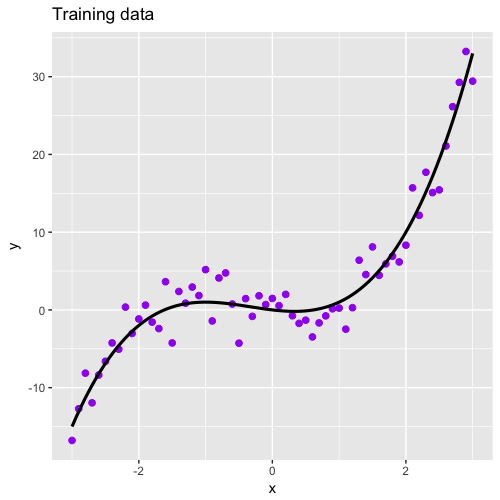
\includegraphics[width=0.40000\textwidth]{Prob1f1.png}
\caption{\(f(x)=-x+x^2+x^3\)}
\end{figure}

In real life we are presented with a data set of pairs \((x_i,y_i)\),
\(i=1,\ldots,n\), and asked to provide a prediction at a value \(x\). We
will use the method of K nearest neighbour regression to do this here.

We have a training set of \(n=61\) observations \((x_i,y_i)\),
\(i=1,\ldots,n\). The KNN regression method provides a prediction at a
value \(x\) by finding the closes \(K\) points and calculating the
average of the observed \(y\) values at these points.

\[\hat{f}(x_0)=\frac{1}{K}\sum_{i\in \mathcal{N}_0} y_i\]

Given an integer \(K\) and a test observation \(x_0\), the KNN
regression first identifies the \(K\) points in the training data that
are closest (Euclidean distance) to \(x_0\), represented by
\(\mathcal{N}_0\). It then estimates the regression curve at \(x_0\) as
the average of the response values for the training observations in
\(\mathcal{N}_0\).

In addition we have a test set of \(n=61\) observations (at the same
grid points as for the training set), but now with new observed values
\(y\).

We have considered \(K=1,\ldots,25\) in the KNN method. Our experiment
has been repeated \(M=1000\) times (that is, \(M\) versions of training
and test set).

\subsection{a) Training and test MSE}\label{a-training-and-test-mse}

\begin{figure}
\centering
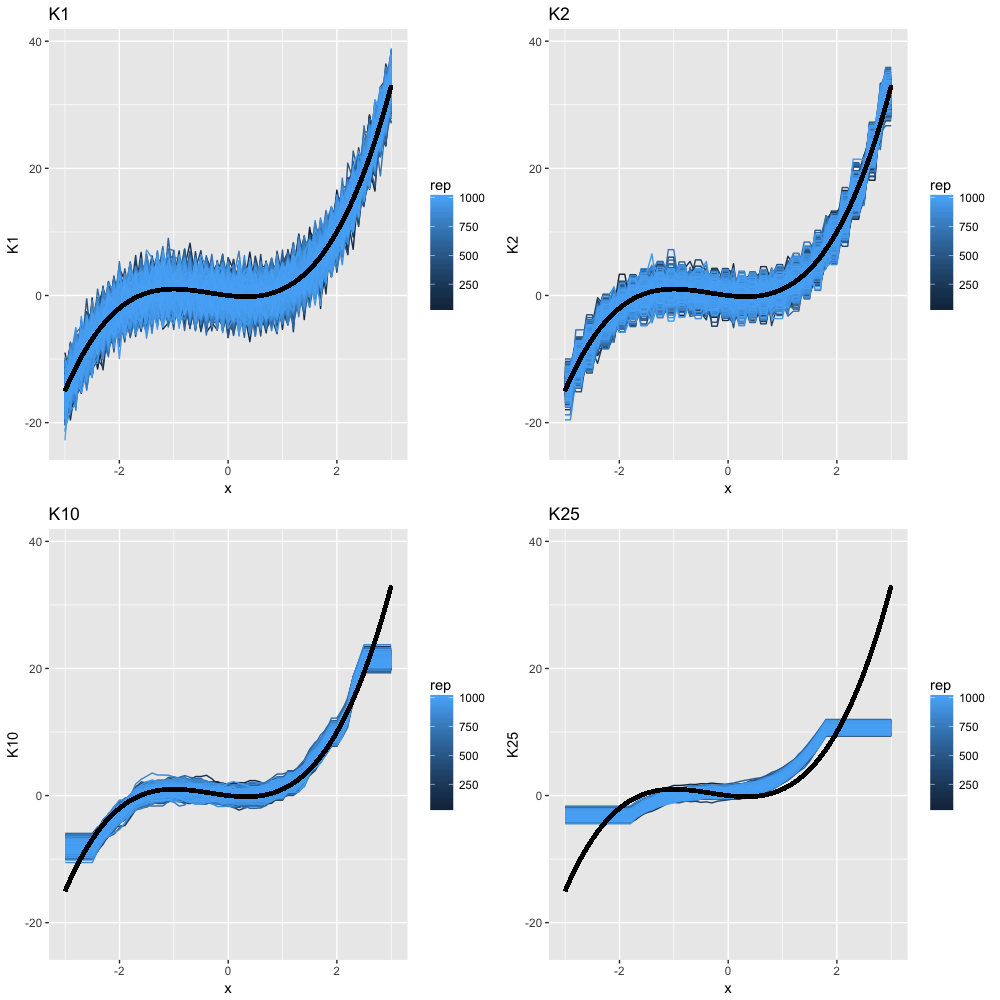
\includegraphics[width=0.80000\textwidth]{Prob1f2.png}
\caption{Figure 2}
\end{figure}

In the Figure 2 (above) you see the result of applying the KNN method
with \(K=1,2,10,25\) to our training data, repeated for \(M\) different
training sets (blue lines). The black lines show the true underlying
curve.

\begin{itemize}
\tightlist
\item
  Comment briefly on what you see.
\item
  Does a high or low value of \(K\) give the most flexible fit?
\end{itemize}

In Figure 3 (below) you see mean-squared errors (mean of squared
differences between observed and fitted values) for the training set and
for the test set (right panel for one training and one test set, and
left panel for \(M\)).

\begin{itemize}
\tightlist
\item
  Comment on what you see.
\item
  What do you think is the ``best'' choice for K?
\end{itemize}

Remark: in real life we do not know the true curve, and need to use the
test data to decide on model flexibility (choosing \(K\)).

\begin{figure}
\centering
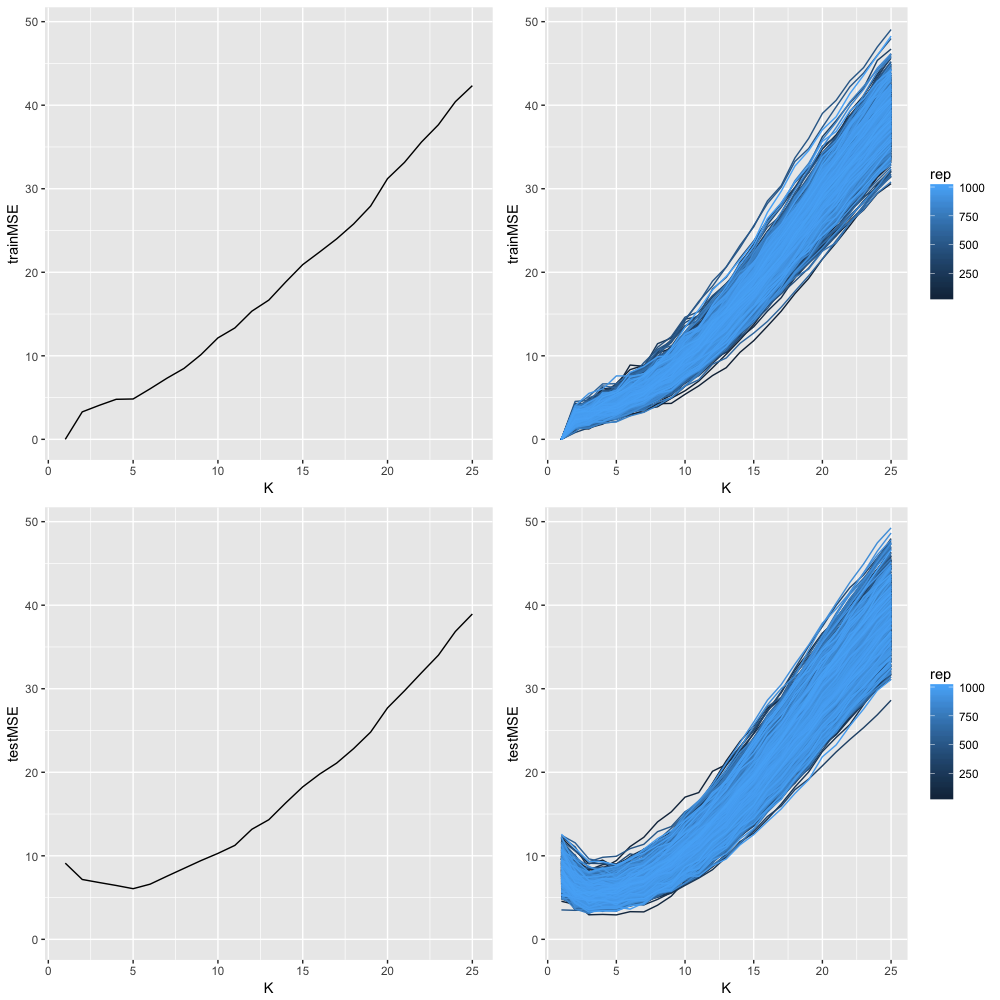
\includegraphics[width=0.80000\textwidth]{Prob1f3.png}
\caption{Mean squared errors for training and test sets}
\end{figure}

\subsection{b) Bias-variance trade-off}\label{b-bias-variance-trade-off}

Now we leave the real world situation, and assume we know the truth
(this is to focus on bias-variance trade-off). You will not observe
these curves in real life - but the understanding of the bias-variance
trade-off is a core skill in this course!

In the Figure 4 (below) you see a plot of estimated squared bias,
estimated variance, true irreducible error and the sum of these
(labelled total) and averaged over all values of \(x\)

The the squared bias and the variance is calculated based on the
predicted values and the ``true'' values (without the added noise) at
each \(x\).

\begin{itemize}
\tightlist
\item
  Explain how that is done. Hint: this is what the \(M\) repeated
  training data sets are used for.
\item
  Focus on Figure 4. As the flexibility of the model increases (\(K\)
  decreases), what happens with

  \begin{itemize}
  \tightlist
  \item
    the squared bias,\\
  \item
    the variance, and\\
  \item
    the irreducible error?
  \end{itemize}
\item
  What would you recommend is the optimal value of \(K\)? Is this in
  agreement with what you found in a)?
\end{itemize}

Extra: We have chosen to also plot curves at four values of \(x\) -
Figure 5 (below). Based on these four curves, that would you recommend
is the optimal value of \(K\)? Is this in agreement with what you found
previously (averaged over \(x\))?

\begin{figure}
\centering
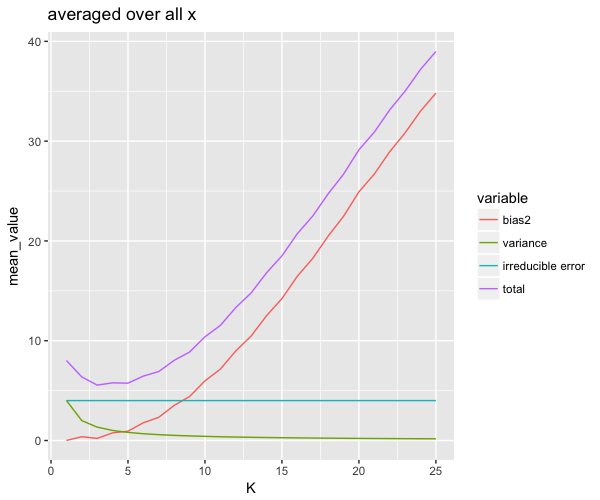
\includegraphics[width=0.60000\textwidth]{Prob1f4.png}
\caption{Figure 4}
\end{figure}

\begin{figure}
\centering
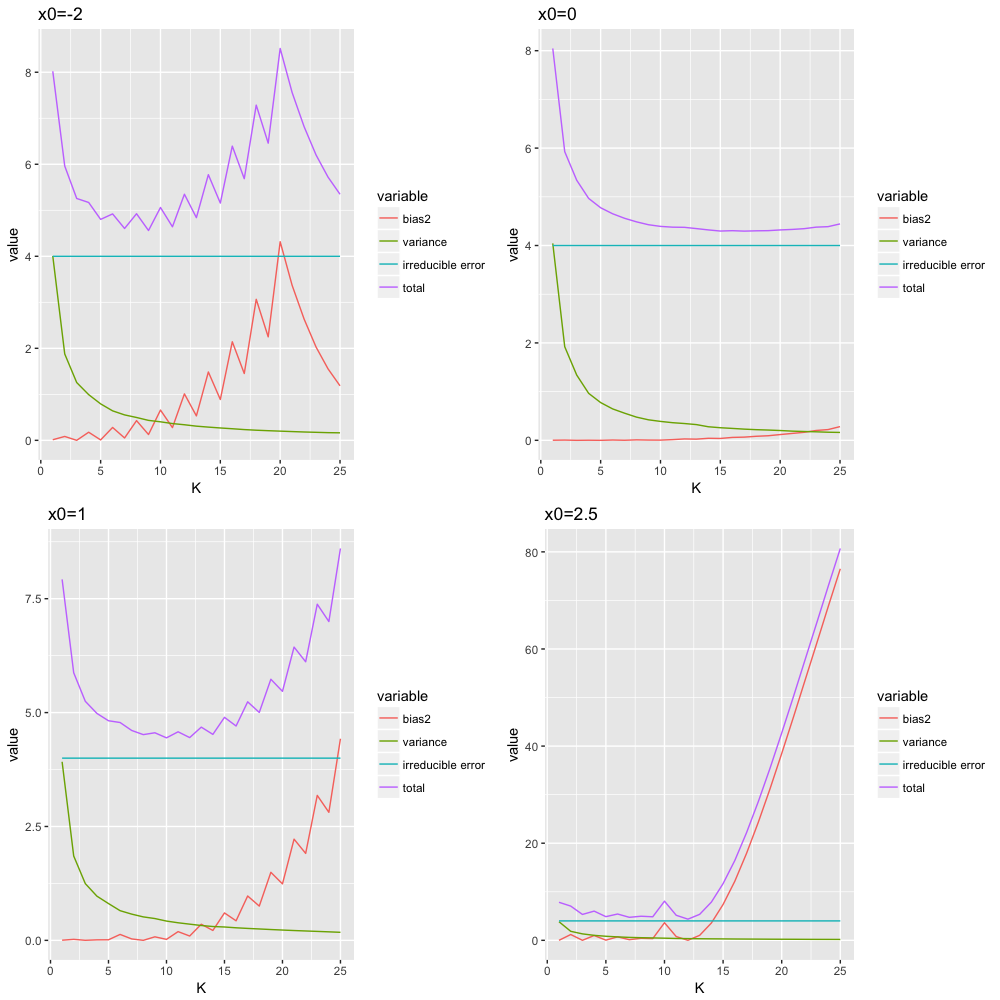
\includegraphics[width=0.80000\textwidth]{Prob1f5.png}
\caption{Figure 5}
\end{figure}

\begin{center}\rule{0.5\linewidth}{\linethickness}\end{center}

For completeness the R code used is given next (listed here with
\texttt{M=100} but \texttt{M=1000} was used). You do not need to run the
code, this is just if you have questions about how this was done.

\footnotesize

\begin{Shaded}
\begin{Highlighting}[]
\KeywordTok{library}\NormalTok{(FNN)}
\KeywordTok{library}\NormalTok{(ggplot2)}
\KeywordTok{library}\NormalTok{(ggpubr)}
\KeywordTok{library}\NormalTok{(reshape2)}
\KeywordTok{library}\NormalTok{(dplyr)}
\NormalTok{maxK =}\StringTok{ }\DecValTok{25}
\NormalTok{M =}\StringTok{ }\DecValTok{1000}  \CommentTok{# repeated samplings, x fixed  - examples were run with M=1000}
\NormalTok{x =}\StringTok{ }\KeywordTok{seq}\NormalTok{(}\OperatorTok{-}\DecValTok{3}\NormalTok{, }\DecValTok{3}\NormalTok{, }\FloatTok{0.1}\NormalTok{)}
\NormalTok{dfx =}\StringTok{ }\KeywordTok{data.frame}\NormalTok{(}\DataTypeTok{x =}\NormalTok{ x)}
\NormalTok{truefunc =}\StringTok{ }\ControlFlowTok{function}\NormalTok{(x) }\KeywordTok{return}\NormalTok{(}\OperatorTok{-}\NormalTok{x }\OperatorTok{+}\StringTok{ }\NormalTok{x}\OperatorTok{^}\DecValTok{2} \OperatorTok{+}\StringTok{ }\NormalTok{x}\OperatorTok{^}\DecValTok{3}\NormalTok{)}
\NormalTok{true_y =}\StringTok{ }\KeywordTok{truefunc}\NormalTok{(x)}

\KeywordTok{set.seed}\NormalTok{(}\DecValTok{2}\NormalTok{)  }\CommentTok{# to reproduce}
\NormalTok{error =}\StringTok{ }\KeywordTok{matrix}\NormalTok{(}\KeywordTok{rnorm}\NormalTok{(}\KeywordTok{length}\NormalTok{(x) }\OperatorTok{*}\StringTok{ }\NormalTok{M, }\DataTypeTok{mean =} \DecValTok{0}\NormalTok{, }\DataTypeTok{sd =} \DecValTok{2}\NormalTok{), }\DataTypeTok{nrow =}\NormalTok{ M, }\DataTypeTok{byrow =} \OtherTok{TRUE}\NormalTok{)}
\NormalTok{testerror =}\StringTok{ }\KeywordTok{matrix}\NormalTok{(}\KeywordTok{rnorm}\NormalTok{(}\KeywordTok{length}\NormalTok{(x) }\OperatorTok{*}\StringTok{ }\NormalTok{M, }\DataTypeTok{mean =} \DecValTok{0}\NormalTok{, }\DataTypeTok{sd =} \DecValTok{2}\NormalTok{), }\DataTypeTok{nrow =}\NormalTok{ M, }
    \DataTypeTok{byrow =} \OtherTok{TRUE}\NormalTok{)}
\NormalTok{ymat =}\StringTok{ }\KeywordTok{matrix}\NormalTok{(}\KeywordTok{rep}\NormalTok{(true_y, M), }\DataTypeTok{byrow =}\NormalTok{ T, }\DataTypeTok{nrow =}\NormalTok{ M) }\OperatorTok{+}\StringTok{ }\NormalTok{error}
\NormalTok{testymat =}\StringTok{ }\KeywordTok{matrix}\NormalTok{(}\KeywordTok{rep}\NormalTok{(true_y, M), }\DataTypeTok{byrow =}\NormalTok{ T, }\DataTypeTok{nrow =}\NormalTok{ M) }\OperatorTok{+}\StringTok{ }\NormalTok{testerror}

\KeywordTok{ggplot}\NormalTok{(}\DataTypeTok{data =} \KeywordTok{data.frame}\NormalTok{(}\DataTypeTok{x =}\NormalTok{ x, }\DataTypeTok{y =}\NormalTok{ ymat[}\DecValTok{1}\NormalTok{, ]), }\KeywordTok{aes}\NormalTok{(x, y)) }\OperatorTok{+}\StringTok{ }\KeywordTok{geom_point}\NormalTok{(}\DataTypeTok{col =} \StringTok{"purple"}\NormalTok{, }
    \DataTypeTok{size =} \DecValTok{2}\NormalTok{) }\OperatorTok{+}\StringTok{ }\KeywordTok{stat_function}\NormalTok{(}\DataTypeTok{fun =}\NormalTok{ truefunc, }\DataTypeTok{lwd =} \FloatTok{1.1}\NormalTok{, }\DataTypeTok{colour =} \StringTok{"black"}\NormalTok{) }\OperatorTok{+}\StringTok{ }
\StringTok{    }\KeywordTok{ggtitle}\NormalTok{(}\StringTok{"Training data"}\NormalTok{)}

\NormalTok{predarray =}\StringTok{ }\KeywordTok{array}\NormalTok{(}\OtherTok{NA}\NormalTok{, }\DataTypeTok{dim =} \KeywordTok{c}\NormalTok{(M, }\KeywordTok{length}\NormalTok{(x), maxK))}
\ControlFlowTok{for}\NormalTok{ (i }\ControlFlowTok{in} \DecValTok{1}\OperatorTok{:}\NormalTok{M) \{}
    \ControlFlowTok{for}\NormalTok{ (j }\ControlFlowTok{in} \DecValTok{1}\OperatorTok{:}\NormalTok{maxK) \{}
\NormalTok{        predarray[i, , j] =}\StringTok{ }\KeywordTok{knn.reg}\NormalTok{(}\DataTypeTok{train =}\NormalTok{ dfx, }\DataTypeTok{test =}\NormalTok{ dfx, }\DataTypeTok{y =} \KeywordTok{c}\NormalTok{(ymat[i, }
\NormalTok{            ]), }\DataTypeTok{k =}\NormalTok{ j)}\OperatorTok{$}\NormalTok{pred}
\NormalTok{    \}}
\NormalTok{\}}
\CommentTok{# first - just plot the fitted values - and add the true curve in}
\CommentTok{# black M curves and choose k=1,2,10,30 in KNN}

\CommentTok{# rearranging to get data frame that is useful}
\NormalTok{thislwd =}\StringTok{ }\FloatTok{1.3}
\NormalTok{stackmat =}\StringTok{ }\OtherTok{NULL}
\ControlFlowTok{for}\NormalTok{ (i }\ControlFlowTok{in} \DecValTok{1}\OperatorTok{:}\NormalTok{M) stackmat =}\StringTok{ }\KeywordTok{rbind}\NormalTok{(stackmat, }\KeywordTok{cbind}\NormalTok{(x, }\KeywordTok{rep}\NormalTok{(i, }\KeywordTok{length}\NormalTok{(x)), }
\NormalTok{    predarray[i, , ]))}
\KeywordTok{colnames}\NormalTok{(stackmat) =}\StringTok{ }\KeywordTok{c}\NormalTok{(}\StringTok{"x"}\NormalTok{, }\StringTok{"rep"}\NormalTok{, }\KeywordTok{paste}\NormalTok{(}\StringTok{"K"}\NormalTok{, }\DecValTok{1}\OperatorTok{:}\NormalTok{maxK, }\DataTypeTok{sep =} \StringTok{""}\NormalTok{))}
\NormalTok{sdf =}\StringTok{ }\KeywordTok{as.data.frame}\NormalTok{(stackmat)}
\NormalTok{yrange =}\StringTok{ }\KeywordTok{range}\NormalTok{(}\KeywordTok{apply}\NormalTok{(sdf, }\DecValTok{2}\NormalTok{, range)[, }\DecValTok{3}\OperatorTok{:}\NormalTok{(maxK }\OperatorTok{+}\StringTok{ }\DecValTok{2}\NormalTok{)])}
\CommentTok{# making the four selected plots}
\NormalTok{p1 =}\StringTok{ }\KeywordTok{ggplot}\NormalTok{(}\DataTypeTok{data =}\NormalTok{ sdf, }\KeywordTok{aes}\NormalTok{(}\DataTypeTok{x =}\NormalTok{ x, }\DataTypeTok{y =}\NormalTok{ K1, }\DataTypeTok{group =}\NormalTok{ rep, }\DataTypeTok{colour =}\NormalTok{ rep)) }\OperatorTok{+}\StringTok{ }
\StringTok{    }\KeywordTok{scale_y_continuous}\NormalTok{(}\DataTypeTok{limits =}\NormalTok{ yrange) }\OperatorTok{+}\StringTok{ }\KeywordTok{geom_line}\NormalTok{()}
\NormalTok{p1 =}\StringTok{ }\NormalTok{p1 }\OperatorTok{+}\StringTok{ }\KeywordTok{stat_function}\NormalTok{(}\DataTypeTok{fun =}\NormalTok{ truefunc, }\DataTypeTok{lwd =}\NormalTok{ thislwd, }\DataTypeTok{colour =} \StringTok{"black"}\NormalTok{) }\OperatorTok{+}\StringTok{ }
\StringTok{    }\KeywordTok{ggtitle}\NormalTok{(}\StringTok{"K1"}\NormalTok{)}
\NormalTok{p2 =}\StringTok{ }\KeywordTok{ggplot}\NormalTok{(}\DataTypeTok{data =}\NormalTok{ sdf, }\KeywordTok{aes}\NormalTok{(}\DataTypeTok{x =}\NormalTok{ x, }\DataTypeTok{y =}\NormalTok{ K2, }\DataTypeTok{group =}\NormalTok{ rep, }\DataTypeTok{colour =}\NormalTok{ rep)) }\OperatorTok{+}\StringTok{ }
\StringTok{    }\KeywordTok{scale_y_continuous}\NormalTok{(}\DataTypeTok{limits =}\NormalTok{ yrange) }\OperatorTok{+}\StringTok{ }\KeywordTok{geom_line}\NormalTok{()}
\NormalTok{p2 =}\StringTok{ }\NormalTok{p2 }\OperatorTok{+}\StringTok{ }\KeywordTok{stat_function}\NormalTok{(}\DataTypeTok{fun =}\NormalTok{ truefunc, }\DataTypeTok{lwd =}\NormalTok{ thislwd, }\DataTypeTok{colour =} \StringTok{"black"}\NormalTok{) }\OperatorTok{+}\StringTok{ }
\StringTok{    }\KeywordTok{ggtitle}\NormalTok{(}\StringTok{"K2"}\NormalTok{)}
\NormalTok{p10 =}\StringTok{ }\KeywordTok{ggplot}\NormalTok{(}\DataTypeTok{data =}\NormalTok{ sdf, }\KeywordTok{aes}\NormalTok{(}\DataTypeTok{x =}\NormalTok{ x, }\DataTypeTok{y =}\NormalTok{ K10, }\DataTypeTok{group =}\NormalTok{ rep, }\DataTypeTok{colour =}\NormalTok{ rep)) }\OperatorTok{+}\StringTok{ }
\StringTok{    }\KeywordTok{scale_y_continuous}\NormalTok{(}\DataTypeTok{limits =}\NormalTok{ yrange) }\OperatorTok{+}\StringTok{ }\KeywordTok{geom_line}\NormalTok{()}
\NormalTok{p10 =}\StringTok{ }\NormalTok{p10 }\OperatorTok{+}\StringTok{ }\KeywordTok{stat_function}\NormalTok{(}\DataTypeTok{fun =}\NormalTok{ truefunc, }\DataTypeTok{lwd =}\NormalTok{ thislwd, }\DataTypeTok{colour =} \StringTok{"black"}\NormalTok{) }\OperatorTok{+}\StringTok{ }
\StringTok{    }\KeywordTok{ggtitle}\NormalTok{(}\StringTok{"K10"}\NormalTok{)}
\NormalTok{p25 =}\StringTok{ }\KeywordTok{ggplot}\NormalTok{(}\DataTypeTok{data =}\NormalTok{ sdf, }\KeywordTok{aes}\NormalTok{(}\DataTypeTok{x =}\NormalTok{ x, }\DataTypeTok{y =}\NormalTok{ K25, }\DataTypeTok{group =}\NormalTok{ rep, }\DataTypeTok{colour =}\NormalTok{ rep)) }\OperatorTok{+}\StringTok{ }
\StringTok{    }\KeywordTok{scale_y_continuous}\NormalTok{(}\DataTypeTok{limits =}\NormalTok{ yrange) }\OperatorTok{+}\StringTok{ }\KeywordTok{geom_line}\NormalTok{()}
\NormalTok{p25 =}\StringTok{ }\NormalTok{p25 }\OperatorTok{+}\StringTok{ }\KeywordTok{stat_function}\NormalTok{(}\DataTypeTok{fun =}\NormalTok{ truefunc, }\DataTypeTok{lwd =}\NormalTok{ thislwd, }\DataTypeTok{colour =} \StringTok{"black"}\NormalTok{) }\OperatorTok{+}\StringTok{ }
\StringTok{    }\KeywordTok{ggtitle}\NormalTok{(}\StringTok{"K30"}\NormalTok{)}
\KeywordTok{ggarrange}\NormalTok{(p1, p2, p10, p25)}

\CommentTok{# calculating trainMSE and testMSE}
\NormalTok{trainMSE =}\StringTok{ }\KeywordTok{matrix}\NormalTok{(}\DataTypeTok{ncol =}\NormalTok{ maxK, }\DataTypeTok{nrow =}\NormalTok{ M)}
\ControlFlowTok{for}\NormalTok{ (i }\ControlFlowTok{in} \DecValTok{1}\OperatorTok{:}\NormalTok{M) trainMSE[i, ] =}\StringTok{ }\KeywordTok{apply}\NormalTok{((predarray[i, , ] }\OperatorTok{-}\StringTok{ }\NormalTok{ymat[i, ])}\OperatorTok{^}\DecValTok{2}\NormalTok{, }
    \DecValTok{2}\NormalTok{, mean)}
\NormalTok{testMSE =}\StringTok{ }\KeywordTok{matrix}\NormalTok{(}\DataTypeTok{ncol =}\NormalTok{ maxK, }\DataTypeTok{nrow =}\NormalTok{ M)}
\ControlFlowTok{for}\NormalTok{ (i }\ControlFlowTok{in} \DecValTok{1}\OperatorTok{:}\NormalTok{M) testMSE[i, ] =}\StringTok{ }\KeywordTok{apply}\NormalTok{((predarray[i, , ] }\OperatorTok{-}\StringTok{ }\NormalTok{testymat[i, ])}\OperatorTok{^}\DecValTok{2}\NormalTok{, }
    \DecValTok{2}\NormalTok{, mean)}
\CommentTok{# rearranging to get data frame that is useful}
\NormalTok{stackmat =}\StringTok{ }\OtherTok{NULL}
\ControlFlowTok{for}\NormalTok{ (i }\ControlFlowTok{in} \DecValTok{1}\OperatorTok{:}\NormalTok{M) stackmat =}\StringTok{ }\KeywordTok{rbind}\NormalTok{(stackmat, }\KeywordTok{cbind}\NormalTok{(}\KeywordTok{rep}\NormalTok{(i, maxK), }\DecValTok{1}\OperatorTok{:}\NormalTok{maxK, }
\NormalTok{    trainMSE[i, ], testMSE[i, ]))}
\KeywordTok{colnames}\NormalTok{(stackmat) =}\StringTok{ }\KeywordTok{c}\NormalTok{(}\StringTok{"rep"}\NormalTok{, }\StringTok{"K"}\NormalTok{, }\StringTok{"trainMSE"}\NormalTok{, }\StringTok{"testMSE"}\NormalTok{)}
\NormalTok{sdf =}\StringTok{ }\KeywordTok{as.data.frame}\NormalTok{(stackmat)}
\NormalTok{yrange =}\StringTok{ }\KeywordTok{range}\NormalTok{(sdf[, }\DecValTok{3}\OperatorTok{:}\DecValTok{4}\NormalTok{])}
\CommentTok{# plotting training and test MSE}
\NormalTok{p1 =}\StringTok{ }\KeywordTok{ggplot}\NormalTok{(}\DataTypeTok{data =}\NormalTok{ sdf[}\DecValTok{1}\OperatorTok{:}\NormalTok{maxK, ], }\KeywordTok{aes}\NormalTok{(}\DataTypeTok{x =}\NormalTok{ K, }\DataTypeTok{y =}\NormalTok{ trainMSE)) }\OperatorTok{+}\StringTok{ }\KeywordTok{scale_y_continuous}\NormalTok{(}\DataTypeTok{limits =}\NormalTok{ yrange) }\OperatorTok{+}\StringTok{ }
\StringTok{    }\KeywordTok{geom_line}\NormalTok{()}
\NormalTok{pall =}\StringTok{ }\KeywordTok{ggplot}\NormalTok{(}\DataTypeTok{data =}\NormalTok{ sdf, }\KeywordTok{aes}\NormalTok{(}\DataTypeTok{x =}\NormalTok{ K, }\DataTypeTok{group =}\NormalTok{ rep, }\DataTypeTok{y =}\NormalTok{ trainMSE, }\DataTypeTok{colour =}\NormalTok{ rep)) }\OperatorTok{+}\StringTok{ }
\StringTok{    }\KeywordTok{scale_y_continuous}\NormalTok{(}\DataTypeTok{limits =}\NormalTok{ yrange) }\OperatorTok{+}\StringTok{ }\KeywordTok{geom_line}\NormalTok{()}
\NormalTok{testp1 =}\StringTok{ }\KeywordTok{ggplot}\NormalTok{(}\DataTypeTok{data =}\NormalTok{ sdf[}\DecValTok{1}\OperatorTok{:}\NormalTok{maxK, ], }\KeywordTok{aes}\NormalTok{(}\DataTypeTok{x =}\NormalTok{ K, }\DataTypeTok{y =}\NormalTok{ testMSE)) }\OperatorTok{+}\StringTok{ }\KeywordTok{scale_y_continuous}\NormalTok{(}\DataTypeTok{limits =}\NormalTok{ yrange) }\OperatorTok{+}\StringTok{ }
\StringTok{    }\KeywordTok{geom_line}\NormalTok{()}
\NormalTok{testpall =}\StringTok{ }\KeywordTok{ggplot}\NormalTok{(}\DataTypeTok{data =}\NormalTok{ sdf, }\KeywordTok{aes}\NormalTok{(}\DataTypeTok{x =}\NormalTok{ K, }\DataTypeTok{group =}\NormalTok{ rep, }\DataTypeTok{y =}\NormalTok{ testMSE, }\DataTypeTok{colour =}\NormalTok{ rep)) }\OperatorTok{+}\StringTok{ }
\StringTok{    }\KeywordTok{scale_y_continuous}\NormalTok{(}\DataTypeTok{limits =}\NormalTok{ yrange) }\OperatorTok{+}\StringTok{ }\KeywordTok{geom_line}\NormalTok{()}
\KeywordTok{ggarrange}\NormalTok{(p1, pall, testp1, testpall)}

\CommentTok{# calculating bias^2 and variance}
\NormalTok{meanmat =}\StringTok{ }\KeywordTok{matrix}\NormalTok{(}\DataTypeTok{ncol =} \KeywordTok{length}\NormalTok{(x), }\DataTypeTok{nrow =}\NormalTok{ maxK)}
\NormalTok{varmat =}\StringTok{ }\KeywordTok{matrix}\NormalTok{(}\DataTypeTok{ncol =} \KeywordTok{length}\NormalTok{(x), }\DataTypeTok{nrow =}\NormalTok{ maxK)}
\ControlFlowTok{for}\NormalTok{ (j }\ControlFlowTok{in} \DecValTok{1}\OperatorTok{:}\NormalTok{maxK) \{}
\NormalTok{    meanmat[j, ] =}\StringTok{ }\KeywordTok{apply}\NormalTok{(predarray[, , j], }\DecValTok{2}\NormalTok{, mean)  }\CommentTok{# we now take the mean over the M simulations - to mimic E and Var at each x value and each KNN model}
\NormalTok{    varmat[j, ] =}\StringTok{ }\KeywordTok{apply}\NormalTok{(predarray[, , j], }\DecValTok{2}\NormalTok{, var)}
\NormalTok{\}}
\NormalTok{bias2mat =}\StringTok{ }\NormalTok{(meanmat }\OperatorTok{-}\StringTok{ }\KeywordTok{matrix}\NormalTok{(}\KeywordTok{rep}\NormalTok{(true_y, maxK), }\DataTypeTok{byrow =} \OtherTok{TRUE}\NormalTok{, }\DataTypeTok{nrow =}\NormalTok{ maxK))}\OperatorTok{^}\DecValTok{2}  \CommentTok{#here the truth is finally used!}

\CommentTok{# preparing to plot}
\NormalTok{df =}\StringTok{ }\KeywordTok{data.frame}\NormalTok{(}\KeywordTok{rep}\NormalTok{(x, }\DataTypeTok{each =}\NormalTok{ maxK), }\KeywordTok{rep}\NormalTok{(}\DecValTok{1}\OperatorTok{:}\NormalTok{maxK, }\KeywordTok{length}\NormalTok{(x)), }\KeywordTok{c}\NormalTok{(bias2mat), }
    \KeywordTok{c}\NormalTok{(varmat), }\KeywordTok{rep}\NormalTok{(}\DecValTok{4}\NormalTok{, }\KeywordTok{prod}\NormalTok{(}\KeywordTok{dim}\NormalTok{(varmat))))  }\CommentTok{#irr is just 4}
\KeywordTok{colnames}\NormalTok{(df) =}\StringTok{ }\KeywordTok{c}\NormalTok{(}\StringTok{"x"}\NormalTok{, }\StringTok{"K"}\NormalTok{, }\StringTok{"bias2"}\NormalTok{, }\StringTok{"variance"}\NormalTok{, }\StringTok{"irreducible error"}\NormalTok{)  }\CommentTok{#suitable for plotting}
\NormalTok{df}\OperatorTok{$}\NormalTok{total =}\StringTok{ }\NormalTok{df}\OperatorTok{$}\NormalTok{bias2 }\OperatorTok{+}\StringTok{ }\NormalTok{df}\OperatorTok{$}\NormalTok{variance }\OperatorTok{+}\StringTok{ }\NormalTok{df}\OperatorTok{$}\StringTok{`}\DataTypeTok{irreducible error}\StringTok{`}
\NormalTok{hdf =}\StringTok{ }\KeywordTok{melt}\NormalTok{(df, }\DataTypeTok{id =} \KeywordTok{c}\NormalTok{(}\StringTok{"x"}\NormalTok{, }\StringTok{"K"}\NormalTok{))}
\CommentTok{# averaged over all x - to compare to train and test MSE}
\NormalTok{hdfmean =}\StringTok{ }\NormalTok{hdf }\OperatorTok\StringTok{ }\KeywordTok{group_by}\NormalTok{(K, variable) }\OperatorTok\StringTok{ }\KeywordTok{summarise}\NormalTok{(}\DataTypeTok{mean_value =} \KeywordTok{mean}\NormalTok{(value))}
\KeywordTok{ggplot}\NormalTok{(}\DataTypeTok{data =}\NormalTok{ hdfmean[hdfmean[, }\DecValTok{1}\NormalTok{] }\OperatorTok{<}\StringTok{ }\DecValTok{31}\NormalTok{, ], }\KeywordTok{aes}\NormalTok{(}\DataTypeTok{x =}\NormalTok{ K, }\DataTypeTok{y =}\NormalTok{ mean_value, }
    \DataTypeTok{colour =}\NormalTok{ variable)) }\OperatorTok{+}\StringTok{ }\KeywordTok{geom_line}\NormalTok{() }\OperatorTok{+}\StringTok{ }\KeywordTok{ggtitle}\NormalTok{(}\StringTok{"averaged over all x"}\NormalTok{)}

\CommentTok{# extra: what about different values of x?}
\NormalTok{hdfatxa =}\StringTok{ }\NormalTok{hdf[hdf}\OperatorTok{$}\NormalTok{x }\OperatorTok{==}\StringTok{ }\DecValTok{-2}\NormalTok{, ]}
\NormalTok{hdfatxb =}\StringTok{ }\NormalTok{hdf[hdf}\OperatorTok{$}\NormalTok{x }\OperatorTok{==}\StringTok{ }\DecValTok{0}\NormalTok{, ]}
\NormalTok{hdfatxc =}\StringTok{ }\NormalTok{hdf[hdf}\OperatorTok{$}\NormalTok{x }\OperatorTok{==}\StringTok{ }\DecValTok{1}\NormalTok{, ]}
\NormalTok{hdfatxd =}\StringTok{ }\NormalTok{hdf[hdf}\OperatorTok{$}\NormalTok{x }\OperatorTok{==}\StringTok{ }\FloatTok{2.5}\NormalTok{, ]}
\NormalTok{pa =}\StringTok{ }\KeywordTok{ggplot}\NormalTok{(}\DataTypeTok{data =}\NormalTok{ hdfatxa, }\KeywordTok{aes}\NormalTok{(}\DataTypeTok{x =}\NormalTok{ K, }\DataTypeTok{y =}\NormalTok{ value, }\DataTypeTok{colour =}\NormalTok{ variable)) }\OperatorTok{+}\StringTok{ }
\StringTok{    }\KeywordTok{geom_line}\NormalTok{() }\OperatorTok{+}\StringTok{ }\KeywordTok{ggtitle}\NormalTok{(}\StringTok{"x0=-2"}\NormalTok{)}
\NormalTok{pb =}\StringTok{ }\KeywordTok{ggplot}\NormalTok{(}\DataTypeTok{data =}\NormalTok{ hdfatxb, }\KeywordTok{aes}\NormalTok{(}\DataTypeTok{x =}\NormalTok{ K, }\DataTypeTok{y =}\NormalTok{ value, }\DataTypeTok{colour =}\NormalTok{ variable)) }\OperatorTok{+}\StringTok{ }
\StringTok{    }\KeywordTok{geom_line}\NormalTok{() }\OperatorTok{+}\StringTok{ }\KeywordTok{ggtitle}\NormalTok{(}\StringTok{"x0=0"}\NormalTok{)}
\NormalTok{pc =}\StringTok{ }\KeywordTok{ggplot}\NormalTok{(}\DataTypeTok{data =}\NormalTok{ hdfatxc, }\KeywordTok{aes}\NormalTok{(}\DataTypeTok{x =}\NormalTok{ K, }\DataTypeTok{y =}\NormalTok{ value, }\DataTypeTok{colour =}\NormalTok{ variable)) }\OperatorTok{+}\StringTok{ }
\StringTok{    }\KeywordTok{geom_line}\NormalTok{() }\OperatorTok{+}\StringTok{ }\KeywordTok{ggtitle}\NormalTok{(}\StringTok{"x0=1"}\NormalTok{)}
\NormalTok{pd =}\StringTok{ }\KeywordTok{ggplot}\NormalTok{(}\DataTypeTok{data =}\NormalTok{ hdfatxd, }\KeywordTok{aes}\NormalTok{(}\DataTypeTok{x =}\NormalTok{ K, }\DataTypeTok{y =}\NormalTok{ value, }\DataTypeTok{colour =}\NormalTok{ variable)) }\OperatorTok{+}\StringTok{ }
\StringTok{    }\KeywordTok{geom_line}\NormalTok{() }\OperatorTok{+}\StringTok{ }\KeywordTok{ggtitle}\NormalTok{(}\StringTok{"x0=2.5"}\NormalTok{)}
\KeywordTok{ggarrange}\NormalTok{(pa, pb, pc, pd)}
\end{Highlighting}
\end{Shaded}

\normalsize

\subsection{Problem 3: Theory and practice - MSEtrain, MSEtest, and
bias-variance}\label{problem-3-theory-and-practice---msetrain-msetest-and-bias-variance}

We will now look closely into the simulations and calculations performed
for the MSEtrain, MSEtest, and bias-variance trade-off in PartA.

\begin{itemize}
\tightlist
\item
  The simulations are based on \(f(x)=x^2\) and normal noise with mean 0
  and standard deviation 2 is added.
\item
  \(x\) is on a 0.1 grid from -2 to 4 (61 values).
\item
  Parametric models of different complexity are fitted - poly1-poly20.
\item
  M=100 simulations are done.
\end{itemize}

The aim of this problem is to understand:

\begin{itemize}
\tightlist
\item
  trainMSE
\item
  testMSE
\item
  bias-variance trade-off
\end{itemize}

\begin{center}\rule{0.5\linewidth}{\linethickness}\end{center}

\subsubsection{a) Problem set-up}\label{a-problem-set-up}

\begin{itemize}
\tightlist
\item
  See the code below. Explain what is done. (You need not understand the
  code in detail.) Run the code.
\item
  We will learn more about the \texttt{lm} function in M 3 - now just
  think of this as fitting a polynomial regression and predict gives the
  fitted curve in our grid points. \texttt{predarray} is just a way to
  save M simulations of 61 gridpoints in x and 20 polynomial models.
\end{itemize}

\begin{Shaded}
\begin{Highlighting}[]
\KeywordTok{library}\NormalTok{(ggplot2)}
\KeywordTok{library}\NormalTok{(ggpubr)}
\KeywordTok{set.seed}\NormalTok{(}\DecValTok{2}\NormalTok{)  }\CommentTok{# to reproduce}

\NormalTok{M =}\StringTok{ }\DecValTok{100}  \CommentTok{# repeated samplings, x fixed }
\NormalTok{nord =}\StringTok{ }\DecValTok{20}  \CommentTok{# order of polynoms}


\NormalTok{x =}\StringTok{ }\KeywordTok{seq}\NormalTok{(}\OperatorTok{-}\DecValTok{2}\NormalTok{, }\DecValTok{4}\NormalTok{, }\FloatTok{0.1}\NormalTok{)}
\NormalTok{truefunc =}\StringTok{ }\ControlFlowTok{function}\NormalTok{(x) }\KeywordTok{return}\NormalTok{(x}\OperatorTok{^}\DecValTok{2}\NormalTok{)}
\NormalTok{true_y =}\StringTok{ }\KeywordTok{truefunc}\NormalTok{(x)}

\NormalTok{error =}\StringTok{ }\KeywordTok{matrix}\NormalTok{(}\KeywordTok{rnorm}\NormalTok{(}\KeywordTok{length}\NormalTok{(x) }\OperatorTok{*}\StringTok{ }\NormalTok{M, }\DataTypeTok{mean =} \DecValTok{0}\NormalTok{, }\DataTypeTok{sd =} \DecValTok{2}\NormalTok{), }\DataTypeTok{nrow =}\NormalTok{ M, }\DataTypeTok{byrow =} \OtherTok{TRUE}\NormalTok{)}
\NormalTok{ymat =}\StringTok{ }\KeywordTok{matrix}\NormalTok{(}\KeywordTok{rep}\NormalTok{(true_y, M), }\DataTypeTok{byrow =}\NormalTok{ T, }\DataTypeTok{nrow =}\NormalTok{ M) }\OperatorTok{+}\StringTok{ }\NormalTok{error}

\NormalTok{predarray =}\StringTok{ }\KeywordTok{array}\NormalTok{(}\OtherTok{NA}\NormalTok{, }\DataTypeTok{dim =} \KeywordTok{c}\NormalTok{(M, }\KeywordTok{length}\NormalTok{(x), nord))}
\ControlFlowTok{for}\NormalTok{ (i }\ControlFlowTok{in} \DecValTok{1}\OperatorTok{:}\NormalTok{M) \{}
    \ControlFlowTok{for}\NormalTok{ (j }\ControlFlowTok{in} \DecValTok{1}\OperatorTok{:}\NormalTok{nord) \{}
\NormalTok{        predarray[i, , j] =}\StringTok{ }\KeywordTok{predict}\NormalTok{(}\KeywordTok{lm}\NormalTok{(ymat[i, ] }\OperatorTok{~}\StringTok{ }\KeywordTok{poly}\NormalTok{(x, j, }\DataTypeTok{raw =} \OtherTok{TRUE}\NormalTok{)))}
\NormalTok{    \}}
\NormalTok{\}}
\CommentTok{# M matrices of size length(x) times nord first, only look at}
\CommentTok{# variablity in the M fits and plot M curves where we had 1}

\CommentTok{# for plotting need to stack the matrices underneath eachother and}
\CommentTok{# make new variable 'rep'}
\NormalTok{stackmat =}\StringTok{ }\OtherTok{NULL}
\ControlFlowTok{for}\NormalTok{ (i }\ControlFlowTok{in} \DecValTok{1}\OperatorTok{:}\NormalTok{M) stackmat =}\StringTok{ }\KeywordTok{rbind}\NormalTok{(stackmat, }\KeywordTok{cbind}\NormalTok{(x, }\KeywordTok{rep}\NormalTok{(i, }\KeywordTok{length}\NormalTok{(x)), }
\NormalTok{    predarray[i, , ]))}
\CommentTok{# dim(stackmat)}
\KeywordTok{colnames}\NormalTok{(stackmat) =}\StringTok{ }\KeywordTok{c}\NormalTok{(}\StringTok{"x"}\NormalTok{, }\StringTok{"rep"}\NormalTok{, }\KeywordTok{paste}\NormalTok{(}\StringTok{"poly"}\NormalTok{, }\DecValTok{1}\OperatorTok{:}\DecValTok{20}\NormalTok{, }\DataTypeTok{sep =} \StringTok{""}\NormalTok{))}
\NormalTok{sdf =}\StringTok{ }\KeywordTok{as.data.frame}\NormalTok{(stackmat)  }\CommentTok{#NB have poly1-20 now - but first only use 1,2,20}
\CommentTok{# to add true curve using stat_function - easiest solution}
\NormalTok{true_x =}\StringTok{ }\NormalTok{x}
\NormalTok{yrange =}\StringTok{ }\KeywordTok{range}\NormalTok{(}\KeywordTok{apply}\NormalTok{(sdf, }\DecValTok{2}\NormalTok{, range)[, }\DecValTok{3}\OperatorTok{:}\DecValTok{22}\NormalTok{])}
\NormalTok{p1 =}\StringTok{ }\KeywordTok{ggplot}\NormalTok{(}\DataTypeTok{data =}\NormalTok{ sdf, }\KeywordTok{aes}\NormalTok{(}\DataTypeTok{x =}\NormalTok{ x, }\DataTypeTok{y =}\NormalTok{ poly1, }\DataTypeTok{group =}\NormalTok{ rep, }\DataTypeTok{colour =}\NormalTok{ rep)) }\OperatorTok{+}\StringTok{ }
\StringTok{    }\KeywordTok{scale_y_continuous}\NormalTok{(}\DataTypeTok{limits =}\NormalTok{ yrange) }\OperatorTok{+}\StringTok{ }\KeywordTok{geom_line}\NormalTok{()}
\NormalTok{p1 =}\StringTok{ }\NormalTok{p1 }\OperatorTok{+}\StringTok{ }\KeywordTok{stat_function}\NormalTok{(}\DataTypeTok{fun =}\NormalTok{ truefunc, }\DataTypeTok{lwd =} \FloatTok{1.3}\NormalTok{, }\DataTypeTok{colour =} \StringTok{"black"}\NormalTok{) }\OperatorTok{+}\StringTok{ }
\StringTok{    }\KeywordTok{ggtitle}\NormalTok{(}\StringTok{"poly1"}\NormalTok{)}
\NormalTok{p2 =}\StringTok{ }\KeywordTok{ggplot}\NormalTok{(}\DataTypeTok{data =}\NormalTok{ sdf, }\KeywordTok{aes}\NormalTok{(}\DataTypeTok{x =}\NormalTok{ x, }\DataTypeTok{y =}\NormalTok{ poly2, }\DataTypeTok{group =}\NormalTok{ rep, }\DataTypeTok{colour =}\NormalTok{ rep)) }\OperatorTok{+}\StringTok{ }
\StringTok{    }\KeywordTok{scale_y_continuous}\NormalTok{(}\DataTypeTok{limits =}\NormalTok{ yrange) }\OperatorTok{+}\StringTok{ }\KeywordTok{geom_line}\NormalTok{()}
\NormalTok{p2 =}\StringTok{ }\NormalTok{p2 }\OperatorTok{+}\StringTok{ }\KeywordTok{stat_function}\NormalTok{(}\DataTypeTok{fun =}\NormalTok{ truefunc, }\DataTypeTok{lwd =} \FloatTok{1.3}\NormalTok{, }\DataTypeTok{colour =} \StringTok{"black"}\NormalTok{) }\OperatorTok{+}\StringTok{ }
\StringTok{    }\KeywordTok{ggtitle}\NormalTok{(}\StringTok{"poly2"}\NormalTok{)}
\NormalTok{p10 =}\StringTok{ }\KeywordTok{ggplot}\NormalTok{(}\DataTypeTok{data =}\NormalTok{ sdf, }\KeywordTok{aes}\NormalTok{(}\DataTypeTok{x =}\NormalTok{ x, }\DataTypeTok{y =}\NormalTok{ poly10, }\DataTypeTok{group =}\NormalTok{ rep, }\DataTypeTok{colour =}\NormalTok{ rep)) }\OperatorTok{+}\StringTok{ }
\StringTok{    }\KeywordTok{scale_y_continuous}\NormalTok{(}\DataTypeTok{limits =}\NormalTok{ yrange) }\OperatorTok{+}\StringTok{ }\KeywordTok{geom_line}\NormalTok{()}
\NormalTok{p10 =}\StringTok{ }\NormalTok{p10 }\OperatorTok{+}\StringTok{ }\KeywordTok{stat_function}\NormalTok{(}\DataTypeTok{fun =}\NormalTok{ truefunc, }\DataTypeTok{lwd =} \FloatTok{1.3}\NormalTok{, }\DataTypeTok{colour =} \StringTok{"black"}\NormalTok{) }\OperatorTok{+}\StringTok{ }
\StringTok{    }\KeywordTok{ggtitle}\NormalTok{(}\StringTok{"poly10"}\NormalTok{)}
\NormalTok{p20 =}\StringTok{ }\KeywordTok{ggplot}\NormalTok{(}\DataTypeTok{data =}\NormalTok{ sdf, }\KeywordTok{aes}\NormalTok{(}\DataTypeTok{x =}\NormalTok{ x, }\DataTypeTok{y =}\NormalTok{ poly20, }\DataTypeTok{group =}\NormalTok{ rep, }\DataTypeTok{colour =}\NormalTok{ rep)) }\OperatorTok{+}\StringTok{ }
\StringTok{    }\KeywordTok{scale_y_continuous}\NormalTok{(}\DataTypeTok{limits =}\NormalTok{ yrange) }\OperatorTok{+}\StringTok{ }\KeywordTok{geom_line}\NormalTok{()}
\NormalTok{p20 =}\StringTok{ }\NormalTok{p20 }\OperatorTok{+}\StringTok{ }\KeywordTok{stat_function}\NormalTok{(}\DataTypeTok{fun =}\NormalTok{ truefunc, }\DataTypeTok{lwd =} \FloatTok{1.3}\NormalTok{, }\DataTypeTok{colour =} \StringTok{"black"}\NormalTok{) }\OperatorTok{+}\StringTok{ }
\StringTok{    }\KeywordTok{ggtitle}\NormalTok{(}\StringTok{"poly20"}\NormalTok{)}
\KeywordTok{ggarrange}\NormalTok{(p1, p2, p10, p20)}
\end{Highlighting}
\end{Shaded}

\begin{center}\rule{0.5\linewidth}{\linethickness}\end{center}

\subsubsection{b) Train and test MSE}\label{b-train-and-test-mse}

\begin{itemize}
\tightlist
\item
  First we produce predictions at each grid point based on our training
  data (\texttt{x} and \texttt{ymat})
\item
  but we also draw new observations to calculate testMSE - see
  \texttt{testymat}
\item
  observe how trainMSE and testMSE is calculated
\item
  run the code
\end{itemize}

\begin{Shaded}
\begin{Highlighting}[]
\KeywordTok{set.seed}\NormalTok{(}\DecValTok{2}\NormalTok{)  }\CommentTok{# to reproduce}

\NormalTok{M =}\StringTok{ }\DecValTok{100}  \CommentTok{# repeated samplings,x fixed but new errors}
\NormalTok{nord =}\StringTok{ }\DecValTok{20}
\NormalTok{x =}\StringTok{ }\KeywordTok{seq}\NormalTok{(}\OperatorTok{-}\DecValTok{2}\NormalTok{, }\DecValTok{4}\NormalTok{, }\FloatTok{0.1}\NormalTok{)}
\NormalTok{truefunc =}\StringTok{ }\ControlFlowTok{function}\NormalTok{(x) }\KeywordTok{return}\NormalTok{(x}\OperatorTok{^}\DecValTok{2}\NormalTok{)}
\NormalTok{true_y =}\StringTok{ }\KeywordTok{truefunc}\NormalTok{(x)}

\NormalTok{error =}\StringTok{ }\KeywordTok{matrix}\NormalTok{(}\KeywordTok{rnorm}\NormalTok{(}\KeywordTok{length}\NormalTok{(x) }\OperatorTok{*}\StringTok{ }\NormalTok{M, }\DataTypeTok{mean =} \DecValTok{0}\NormalTok{, }\DataTypeTok{sd =} \DecValTok{2}\NormalTok{), }\DataTypeTok{nrow =}\NormalTok{ M, }\DataTypeTok{byrow =} \OtherTok{TRUE}\NormalTok{)}
\NormalTok{testerror =}\StringTok{ }\KeywordTok{matrix}\NormalTok{(}\KeywordTok{rnorm}\NormalTok{(}\KeywordTok{length}\NormalTok{(x) }\OperatorTok{*}\StringTok{ }\NormalTok{M, }\DataTypeTok{mean =} \DecValTok{0}\NormalTok{, }\DataTypeTok{sd =} \DecValTok{2}\NormalTok{), }\DataTypeTok{nrow =}\NormalTok{ M, }
    \DataTypeTok{byrow =} \OtherTok{TRUE}\NormalTok{)}
\NormalTok{ymat =}\StringTok{ }\KeywordTok{matrix}\NormalTok{(}\KeywordTok{rep}\NormalTok{(true_y, M), }\DataTypeTok{byrow =}\NormalTok{ T, }\DataTypeTok{nrow =}\NormalTok{ M) }\OperatorTok{+}\StringTok{ }\NormalTok{error}
\NormalTok{testymat =}\StringTok{ }\KeywordTok{matrix}\NormalTok{(}\KeywordTok{rep}\NormalTok{(true_y, M), }\DataTypeTok{byrow =}\NormalTok{ T, }\DataTypeTok{nrow =}\NormalTok{ M) }\OperatorTok{+}\StringTok{ }\NormalTok{testerror}

\NormalTok{predarray =}\StringTok{ }\KeywordTok{array}\NormalTok{(}\OtherTok{NA}\NormalTok{, }\DataTypeTok{dim =} \KeywordTok{c}\NormalTok{(M, }\KeywordTok{length}\NormalTok{(x), nord))}
\ControlFlowTok{for}\NormalTok{ (i }\ControlFlowTok{in} \DecValTok{1}\OperatorTok{:}\NormalTok{M) \{}
    \ControlFlowTok{for}\NormalTok{ (j }\ControlFlowTok{in} \DecValTok{1}\OperatorTok{:}\NormalTok{nord) \{}
\NormalTok{        predarray[i, , j] =}\StringTok{ }\KeywordTok{predict}\NormalTok{(}\KeywordTok{lm}\NormalTok{(ymat[i, ] }\OperatorTok{~}\StringTok{ }\KeywordTok{poly}\NormalTok{(x, j, }\DataTypeTok{raw =} \OtherTok{TRUE}\NormalTok{)))}
\NormalTok{    \}}
\NormalTok{\}}
\NormalTok{trainMSE =}\StringTok{ }\KeywordTok{matrix}\NormalTok{(}\DataTypeTok{ncol =}\NormalTok{ nord, }\DataTypeTok{nrow =}\NormalTok{ M)}
\ControlFlowTok{for}\NormalTok{ (i }\ControlFlowTok{in} \DecValTok{1}\OperatorTok{:}\NormalTok{M) trainMSE[i, ] =}\StringTok{ }\KeywordTok{apply}\NormalTok{((predarray[i, , ] }\OperatorTok{-}\StringTok{ }\NormalTok{ymat[i, ])}\OperatorTok{^}\DecValTok{2}\NormalTok{, }
    \DecValTok{2}\NormalTok{, mean)}
\NormalTok{testMSE =}\StringTok{ }\KeywordTok{matrix}\NormalTok{(}\DataTypeTok{ncol =}\NormalTok{ nord, }\DataTypeTok{nrow =}\NormalTok{ M)}
\ControlFlowTok{for}\NormalTok{ (i }\ControlFlowTok{in} \DecValTok{1}\OperatorTok{:}\NormalTok{M) testMSE[i, ] =}\StringTok{ }\KeywordTok{apply}\NormalTok{((predarray[i, , ] }\OperatorTok{-}\StringTok{ }\NormalTok{testymat[i, ])}\OperatorTok{^}\DecValTok{2}\NormalTok{, }
    \DecValTok{2}\NormalTok{, mean)}
\end{Highlighting}
\end{Shaded}

\begin{itemize}
\tightlist
\item
  Then we plot train and testMSE - first for one train + test data set,
  then for 99 more.
\end{itemize}

\begin{Shaded}
\begin{Highlighting}[]
\KeywordTok{library}\NormalTok{(ggplot2)}
\KeywordTok{library}\NormalTok{(ggpubr)}

\CommentTok{# format suitable for plotting}
\NormalTok{stackmat =}\StringTok{ }\OtherTok{NULL}
\ControlFlowTok{for}\NormalTok{ (i }\ControlFlowTok{in} \DecValTok{1}\OperatorTok{:}\NormalTok{M) stackmat =}\StringTok{ }\KeywordTok{rbind}\NormalTok{(stackmat, }\KeywordTok{cbind}\NormalTok{(}\KeywordTok{rep}\NormalTok{(i, nord), }\DecValTok{1}\OperatorTok{:}\NormalTok{nord, }
\NormalTok{    trainMSE[i, ], testMSE[i, ]))}
\KeywordTok{colnames}\NormalTok{(stackmat) =}\StringTok{ }\KeywordTok{c}\NormalTok{(}\StringTok{"rep"}\NormalTok{, }\StringTok{"poly"}\NormalTok{, }\StringTok{"trainMSE"}\NormalTok{, }\StringTok{"testMSE"}\NormalTok{)}
\NormalTok{sdf =}\StringTok{ }\KeywordTok{as.data.frame}\NormalTok{(stackmat)}
\NormalTok{yrange =}\StringTok{ }\KeywordTok{range}\NormalTok{(sdf[, }\DecValTok{3}\OperatorTok{:}\DecValTok{4}\NormalTok{])}
\NormalTok{p1 =}\StringTok{ }\KeywordTok{ggplot}\NormalTok{(}\DataTypeTok{data =}\NormalTok{ sdf[}\DecValTok{1}\OperatorTok{:}\NormalTok{nord, ], }\KeywordTok{aes}\NormalTok{(}\DataTypeTok{x =}\NormalTok{ poly, }\DataTypeTok{y =}\NormalTok{ trainMSE)) }\OperatorTok{+}\StringTok{ }\KeywordTok{scale_y_continuous}\NormalTok{(}\DataTypeTok{limits =}\NormalTok{ yrange) }\OperatorTok{+}\StringTok{ }
\StringTok{    }\KeywordTok{geom_line}\NormalTok{()}
\NormalTok{pall =}\StringTok{ }\KeywordTok{ggplot}\NormalTok{(}\DataTypeTok{data =}\NormalTok{ sdf, }\KeywordTok{aes}\NormalTok{(}\DataTypeTok{x =}\NormalTok{ poly, }\DataTypeTok{group =}\NormalTok{ rep, }\DataTypeTok{y =}\NormalTok{ trainMSE, }\DataTypeTok{colour =}\NormalTok{ rep)) }\OperatorTok{+}\StringTok{ }
\StringTok{    }\KeywordTok{scale_y_continuous}\NormalTok{(}\DataTypeTok{limits =}\NormalTok{ yrange) }\OperatorTok{+}\StringTok{ }\KeywordTok{geom_line}\NormalTok{()}
\NormalTok{testp1 =}\StringTok{ }\KeywordTok{ggplot}\NormalTok{(}\DataTypeTok{data =}\NormalTok{ sdf[}\DecValTok{1}\OperatorTok{:}\NormalTok{nord, ], }\KeywordTok{aes}\NormalTok{(}\DataTypeTok{x =}\NormalTok{ poly, }\DataTypeTok{y =}\NormalTok{ testMSE)) }\OperatorTok{+}\StringTok{ }\KeywordTok{scale_y_continuous}\NormalTok{(}\DataTypeTok{limits =}\NormalTok{ yrange) }\OperatorTok{+}\StringTok{ }
\StringTok{    }\KeywordTok{geom_line}\NormalTok{()}
\NormalTok{testpall =}\StringTok{ }\KeywordTok{ggplot}\NormalTok{(}\DataTypeTok{data =}\NormalTok{ sdf, }\KeywordTok{aes}\NormalTok{(}\DataTypeTok{x =}\NormalTok{ poly, }\DataTypeTok{group =}\NormalTok{ rep, }\DataTypeTok{y =}\NormalTok{ testMSE, }
    \DataTypeTok{colour =}\NormalTok{ rep)) }\OperatorTok{+}\StringTok{ }\KeywordTok{scale_y_continuous}\NormalTok{(}\DataTypeTok{limits =}\NormalTok{ yrange) }\OperatorTok{+}\StringTok{ }\KeywordTok{geom_line}\NormalTok{()}
\KeywordTok{ggarrange}\NormalTok{(p1, pall, testp1, testpall)}
\end{Highlighting}
\end{Shaded}

\begin{itemize}
\tightlist
\item
  More plots: first boxplot and then mean for train and test MSE
\end{itemize}

\begin{Shaded}
\begin{Highlighting}[]
\KeywordTok{library}\NormalTok{(reshape2)}
\NormalTok{df =}\StringTok{ }\KeywordTok{melt}\NormalTok{(sdf, }\DataTypeTok{id =} \KeywordTok{c}\NormalTok{(}\StringTok{"poly"}\NormalTok{, }\StringTok{"rep"}\NormalTok{))[, }\DecValTok{-2}\NormalTok{]}
\KeywordTok{colnames}\NormalTok{(df)[}\DecValTok{2}\NormalTok{] =}\StringTok{ "MSEtype"}
\KeywordTok{ggplot}\NormalTok{(}\DataTypeTok{data =}\NormalTok{ df, }\KeywordTok{aes}\NormalTok{(}\DataTypeTok{x =} \KeywordTok{as.factor}\NormalTok{(poly), }\DataTypeTok{y =}\NormalTok{ value)) }\OperatorTok{+}\StringTok{ }\KeywordTok{geom_boxplot}\NormalTok{(}\KeywordTok{aes}\NormalTok{(}\DataTypeTok{fill =}\NormalTok{ MSEtype))}
\end{Highlighting}
\end{Shaded}

\begin{Shaded}
\begin{Highlighting}[]
\NormalTok{trainMSEmean =}\StringTok{ }\KeywordTok{apply}\NormalTok{(trainMSE, }\DecValTok{2}\NormalTok{, mean)}
\NormalTok{testMSEmean =}\StringTok{ }\KeywordTok{apply}\NormalTok{(testMSE, }\DecValTok{2}\NormalTok{, mean)}
\NormalTok{meandf =}\StringTok{ }\KeywordTok{melt}\NormalTok{(}\KeywordTok{data.frame}\NormalTok{(}\KeywordTok{cbind}\NormalTok{(}\DataTypeTok{poly =} \DecValTok{1}\OperatorTok{:}\NormalTok{nord, trainMSEmean, testMSEmean)), }
    \DataTypeTok{id =} \StringTok{"poly"}\NormalTok{)}
\KeywordTok{ggplot}\NormalTok{(}\DataTypeTok{data =}\NormalTok{ meandf, }\KeywordTok{aes}\NormalTok{(}\DataTypeTok{x =}\NormalTok{ poly, }\DataTypeTok{y =}\NormalTok{ value, }\DataTypeTok{colour =}\NormalTok{ variable)) }\OperatorTok{+}\StringTok{ }
\StringTok{    }\KeywordTok{geom_line}\NormalTok{()}
\end{Highlighting}
\end{Shaded}

\begin{center}\rule{0.5\linewidth}{\linethickness}\end{center}

\subsubsection{c) Bias and variance - we use the
truth!}\label{c-bias-and-variance---we-use-the-truth}

Finally, we want to see how the expected quadratic loss can be
decomposed into

\begin{itemize}
\tightlist
\item
  irreducible error: \(\text{Var}(\varepsilon)=4\)
\item
  squared bias: difference between mean of estimated parametric model
  chosen and the true underlying curve (\texttt{truefunc})
\item
  variance: variance of the estimated parametric model
\end{itemize}

Notice that the test data is not used - only predicted values in each x
grid point.

Study and run the code. Explain the plots produced.

\begin{Shaded}
\begin{Highlighting}[]
\NormalTok{meanmat =}\StringTok{ }\KeywordTok{matrix}\NormalTok{(}\DataTypeTok{ncol =} \KeywordTok{length}\NormalTok{(x), }\DataTypeTok{nrow =}\NormalTok{ nord)}
\NormalTok{varmat =}\StringTok{ }\KeywordTok{matrix}\NormalTok{(}\DataTypeTok{ncol =} \KeywordTok{length}\NormalTok{(x), }\DataTypeTok{nrow =}\NormalTok{ nord)}
\ControlFlowTok{for}\NormalTok{ (j }\ControlFlowTok{in} \DecValTok{1}\OperatorTok{:}\NormalTok{nord) \{}
\NormalTok{    meanmat[j, ] =}\StringTok{ }\KeywordTok{apply}\NormalTok{(predarray[, , j], }\DecValTok{2}\NormalTok{, mean)  }\CommentTok{# we now take the mean over the M simulations - to mimic E and Var at each x value and each poly model}
\NormalTok{    varmat[j, ] =}\StringTok{ }\KeywordTok{apply}\NormalTok{(predarray[, , j], }\DecValTok{2}\NormalTok{, var)}
\NormalTok{\}}
\CommentTok{# nord times length(x)}
\NormalTok{bias2mat =}\StringTok{ }\NormalTok{(meanmat }\OperatorTok{-}\StringTok{ }\KeywordTok{matrix}\NormalTok{(}\KeywordTok{rep}\NormalTok{(true_y, nord), }\DataTypeTok{byrow =} \OtherTok{TRUE}\NormalTok{, }\DataTypeTok{nrow =}\NormalTok{ nord))}\OperatorTok{^}\DecValTok{2}  \CommentTok{#here the truth is finally used!}
\end{Highlighting}
\end{Shaded}

\begin{itemize}
\tightlist
\item
  Plotting the polys as a function of x
\end{itemize}

\begin{Shaded}
\begin{Highlighting}[]
\NormalTok{df =}\StringTok{ }\KeywordTok{data.frame}\NormalTok{(}\KeywordTok{rep}\NormalTok{(x, }\DataTypeTok{each =}\NormalTok{ nord), }\KeywordTok{rep}\NormalTok{(}\DecValTok{1}\OperatorTok{:}\NormalTok{nord, }\KeywordTok{length}\NormalTok{(x)), }\KeywordTok{c}\NormalTok{(bias2mat), }
    \KeywordTok{c}\NormalTok{(varmat), }\KeywordTok{rep}\NormalTok{(}\DecValTok{4}\NormalTok{, }\KeywordTok{prod}\NormalTok{(}\KeywordTok{dim}\NormalTok{(varmat))))  }\CommentTok{#irr is just 1}
\KeywordTok{colnames}\NormalTok{(df) =}\StringTok{ }\KeywordTok{c}\NormalTok{(}\StringTok{"x"}\NormalTok{, }\StringTok{"poly"}\NormalTok{, }\StringTok{"bias2"}\NormalTok{, }\StringTok{"variance"}\NormalTok{, }\StringTok{"irreducible error"}\NormalTok{)  }\CommentTok{#suitable for plotting}
\NormalTok{df}\OperatorTok{$}\NormalTok{total =}\StringTok{ }\NormalTok{df}\OperatorTok{$}\NormalTok{bias2 }\OperatorTok{+}\StringTok{ }\NormalTok{df}\OperatorTok{$}\NormalTok{variance }\OperatorTok{+}\StringTok{ }\NormalTok{df}\OperatorTok{$}\StringTok{`}\DataTypeTok{irreducible error}\StringTok{`}
\NormalTok{hdf =}\StringTok{ }\KeywordTok{melt}\NormalTok{(df, }\DataTypeTok{id =} \KeywordTok{c}\NormalTok{(}\StringTok{"x"}\NormalTok{, }\StringTok{"poly"}\NormalTok{))}
\NormalTok{hdf1 =}\StringTok{ }\NormalTok{hdf[hdf}\OperatorTok{$}\NormalTok{poly }\OperatorTok{==}\StringTok{ }\DecValTok{1}\NormalTok{, ]}
\NormalTok{hdf2 =}\StringTok{ }\NormalTok{hdf[hdf}\OperatorTok{$}\NormalTok{poly }\OperatorTok{==}\StringTok{ }\DecValTok{2}\NormalTok{, ]}
\NormalTok{hdf10 =}\StringTok{ }\NormalTok{hdf[hdf}\OperatorTok{$}\NormalTok{poly }\OperatorTok{==}\StringTok{ }\DecValTok{10}\NormalTok{, ]}
\NormalTok{hdf20 =}\StringTok{ }\NormalTok{hdf[hdf}\OperatorTok{$}\NormalTok{poly }\OperatorTok{==}\StringTok{ }\DecValTok{20}\NormalTok{, ]}

\NormalTok{p1 =}\StringTok{ }\KeywordTok{ggplot}\NormalTok{(}\DataTypeTok{data =}\NormalTok{ hdf1, }\KeywordTok{aes}\NormalTok{(}\DataTypeTok{x =}\NormalTok{ x, }\DataTypeTok{y =}\NormalTok{ value, }\DataTypeTok{colour =}\NormalTok{ variable)) }\OperatorTok{+}\StringTok{ }
\StringTok{    }\KeywordTok{geom_line}\NormalTok{() }\OperatorTok{+}\StringTok{ }\KeywordTok{ggtitle}\NormalTok{(}\StringTok{"poly1"}\NormalTok{)}
\NormalTok{p2 =}\StringTok{ }\KeywordTok{ggplot}\NormalTok{(}\DataTypeTok{data =}\NormalTok{ hdf2, }\KeywordTok{aes}\NormalTok{(}\DataTypeTok{x =}\NormalTok{ x, }\DataTypeTok{y =}\NormalTok{ value, }\DataTypeTok{colour =}\NormalTok{ variable)) }\OperatorTok{+}\StringTok{ }
\StringTok{    }\KeywordTok{geom_line}\NormalTok{() }\OperatorTok{+}\StringTok{ }\KeywordTok{ggtitle}\NormalTok{(}\StringTok{"poly2"}\NormalTok{)}
\NormalTok{p10 =}\StringTok{ }\KeywordTok{ggplot}\NormalTok{(}\DataTypeTok{data =}\NormalTok{ hdf10, }\KeywordTok{aes}\NormalTok{(}\DataTypeTok{x =}\NormalTok{ x, }\DataTypeTok{y =}\NormalTok{ value, }\DataTypeTok{colour =}\NormalTok{ variable)) }\OperatorTok{+}\StringTok{ }
\StringTok{    }\KeywordTok{geom_line}\NormalTok{() }\OperatorTok{+}\StringTok{ }\KeywordTok{ggtitle}\NormalTok{(}\StringTok{"poly10"}\NormalTok{)}
\NormalTok{p20 =}\StringTok{ }\KeywordTok{ggplot}\NormalTok{(}\DataTypeTok{data =}\NormalTok{ hdf20, }\KeywordTok{aes}\NormalTok{(}\DataTypeTok{x =}\NormalTok{ x, }\DataTypeTok{y =}\NormalTok{ value, }\DataTypeTok{colour =}\NormalTok{ variable)) }\OperatorTok{+}\StringTok{ }
\StringTok{    }\KeywordTok{geom_line}\NormalTok{() }\OperatorTok{+}\StringTok{ }\KeywordTok{ggtitle}\NormalTok{(}\StringTok{"poly20"}\NormalTok{)}
\KeywordTok{ggarrange}\NormalTok{(p1, p2, p10, p20)}
\end{Highlighting}
\end{Shaded}

\begin{itemize}
\tightlist
\item
  Now plotting effect of more complex model at 4 chosen values of x,
  compare to Figures in 2.12 on page 36 in ISL (our textbook).
\end{itemize}

\begin{Shaded}
\begin{Highlighting}[]
\NormalTok{hdfatxa =}\StringTok{ }\NormalTok{hdf[hdf}\OperatorTok{$}\NormalTok{x }\OperatorTok{==}\StringTok{ }\DecValTok{-1}\NormalTok{, ]}
\NormalTok{hdfatxb =}\StringTok{ }\NormalTok{hdf[hdf}\OperatorTok{$}\NormalTok{x }\OperatorTok{==}\StringTok{ }\FloatTok{0.5}\NormalTok{, ]}
\NormalTok{hdfatxc =}\StringTok{ }\NormalTok{hdf[hdf}\OperatorTok{$}\NormalTok{x }\OperatorTok{==}\StringTok{ }\DecValTok{2}\NormalTok{, ]}
\NormalTok{hdfatxd =}\StringTok{ }\NormalTok{hdf[hdf}\OperatorTok{$}\NormalTok{x }\OperatorTok{==}\StringTok{ }\FloatTok{3.5}\NormalTok{, ]}
\NormalTok{pa =}\StringTok{ }\KeywordTok{ggplot}\NormalTok{(}\DataTypeTok{data =}\NormalTok{ hdfatxa, }\KeywordTok{aes}\NormalTok{(}\DataTypeTok{x =}\NormalTok{ poly, }\DataTypeTok{y =}\NormalTok{ value, }\DataTypeTok{colour =}\NormalTok{ variable)) }\OperatorTok{+}\StringTok{ }
\StringTok{    }\KeywordTok{geom_line}\NormalTok{() }\OperatorTok{+}\StringTok{ }\KeywordTok{ggtitle}\NormalTok{(}\StringTok{"x0=-1"}\NormalTok{)}
\NormalTok{pb =}\StringTok{ }\KeywordTok{ggplot}\NormalTok{(}\DataTypeTok{data =}\NormalTok{ hdfatxb, }\KeywordTok{aes}\NormalTok{(}\DataTypeTok{x =}\NormalTok{ poly, }\DataTypeTok{y =}\NormalTok{ value, }\DataTypeTok{colour =}\NormalTok{ variable)) }\OperatorTok{+}\StringTok{ }
\StringTok{    }\KeywordTok{geom_line}\NormalTok{() }\OperatorTok{+}\StringTok{ }\KeywordTok{ggtitle}\NormalTok{(}\StringTok{"x0=0.5"}\NormalTok{)}
\NormalTok{pc =}\StringTok{ }\KeywordTok{ggplot}\NormalTok{(}\DataTypeTok{data =}\NormalTok{ hdfatxc, }\KeywordTok{aes}\NormalTok{(}\DataTypeTok{x =}\NormalTok{ poly, }\DataTypeTok{y =}\NormalTok{ value, }\DataTypeTok{colour =}\NormalTok{ variable)) }\OperatorTok{+}\StringTok{ }
\StringTok{    }\KeywordTok{geom_line}\NormalTok{() }\OperatorTok{+}\StringTok{ }\KeywordTok{ggtitle}\NormalTok{(}\StringTok{"x0=2"}\NormalTok{)}
\NormalTok{pd =}\StringTok{ }\KeywordTok{ggplot}\NormalTok{(}\DataTypeTok{data =}\NormalTok{ hdfatxd, }\KeywordTok{aes}\NormalTok{(}\DataTypeTok{x =}\NormalTok{ poly, }\DataTypeTok{y =}\NormalTok{ value, }\DataTypeTok{colour =}\NormalTok{ variable)) }\OperatorTok{+}\StringTok{ }
\StringTok{    }\KeywordTok{geom_line}\NormalTok{() }\OperatorTok{+}\StringTok{ }\KeywordTok{ggtitle}\NormalTok{(}\StringTok{"x0=3.5"}\NormalTok{)}
\KeywordTok{ggarrange}\NormalTok{(pa, pb, pc, pd)}
\end{Highlighting}
\end{Shaded}

\begin{center}\rule{0.5\linewidth}{\linethickness}\end{center}

\subsubsection{d) Repeat a-c}\label{d-repeat-a-c}

\begin{itemize}
\tightlist
\item
  Then try to change the true function \texttt{truefunc} to something
  else - mayby order 3? What does this do the the plots produced? Maybe
  you then also want to plot poly3?
\item
  Also try to change the standard deviation of the noise added to the
  curve (now it is sd=2). What happens if you change this to sd=1 or
  sd=3?
\item
  Or, change to the true function that is not a polynomial?
\end{itemize}

\begin{center}\rule{0.5\linewidth}{\linethickness}\end{center}

\subsection{Problem 4: An exam problem from
2018}\label{problem-4-an-exam-problem-from-2018}

We have a univariate continuous random variable \(Y\) and a covariate
\(x\). Further, we have observed a training set of independent
observation pairs \(\{x_i, y_i\}\) for \(i=1,\ldots,n\).

Assume a regression model \[Y_i  = f(x_i) + \varepsilon_i\] where \(f\)
is the true regression function, and \(\varepsilon_i\) is an unobserved
random variable with mean zero and constant variance \(\sigma^2\) (not
dependent on the covariate). Using the training set we can find an
estimate of the regression function \(f\), and we denote this by
\(\hat{f}\). We want to use \(\hat{f}\) to make a prediction for a new
observation (not dependent on the observations in the training set) at a
covariate value \(x_0\). The predicted response value is then
\(\hat{f}(x_0)\). We are interested in the error associated with this
prediction.

\textbf{Q5:} Write down the definition of the expected test mean squared
error (MSE) at \(x_0\).

\textbf{Q6:} Derive the decomposition of the expected test MSE into
three terms.

\textbf{Q7:} Explain with words how we can interpret the three terms.

Assume that we have a method to estimate the regression function, where
this method has a tuning parameter that controls the complexity of the
model and that a large value of the tuning parameter gives high model
complexity.

\textbf{Q8:} Make a sketch of how the expected test MSE (at \(x_0\)) and
the decomposition into three terms could look as a function of the
tuning parameter.

This decomposition has played a central role in our course.

\textbf{Q9:} In your opinion, what is the most important implication of
this decomposition? Answer with \emph{only one} sentence.

\section{ Further reading/resources}\label{further-readingresources}

\begin{itemize}
\tightlist
\item
  \href{https://www.youtube.com/playlist?list=PL5-da3qGB5IDvuFPNoSqheihPOQNJpzyy}{Videoes
  on YouTube by the authors of ISL, Chapter 2}
\end{itemize}

\section{ R packages}\label{r-packages}

If you want to look at the .Rmd file and \texttt{knit} it, you need to
first install the following packages (only once).

\begin{Shaded}
\begin{Highlighting}[]
\KeywordTok{install.packages}\NormalTok{(}\StringTok{"knitr"}\NormalTok{)}
\KeywordTok{install.packages}\NormalTok{(}\StringTok{"kableExtra"}\NormalTok{)}
\KeywordTok{install.packages}\NormalTok{(}\StringTok{"rmarkdown"}\NormalTok{)}
\KeywordTok{install.packages}\NormalTok{(}\StringTok{"devtools"}\NormalTok{)}
\KeywordTok{install.packages}\NormalTok{(}\StringTok{"ggplot2"}\NormalTok{)}
\KeywordTok{install.packages}\NormalTok{(}\StringTok{"ggpubr"}\NormalTok{)}
\KeywordTok{install.packages}\NormalTok{(}\StringTok{"dplyr"}\NormalTok{)}
\KeywordTok{install.packages}\NormalTok{(}\StringTok{"reshape2"}\NormalTok{)}
\KeywordTok{install.packages}\NormalTok{(}\StringTok{"ElemStatLearn"}\NormalTok{)}
\KeywordTok{install.packages}\NormalTok{(}\StringTok{"GGally"}\NormalTok{)}
\KeywordTok{install.packages}\NormalTok{(}\StringTok{"class"}\NormalTok{)}
\KeywordTok{install.packages}\NormalTok{(}\StringTok{"mvtnorm"}\NormalTok{)}
\KeywordTok{install.packages}\NormalTok{(}\StringTok{"MASS"}\NormalTok{)}
\KeywordTok{install.packages}\NormalTok{(}\StringTok{"car"}\NormalTok{)}
\KeywordTok{install.packages}\NormalTok{(}\StringTok{"faraway"}\NormalTok{)}
\KeywordTok{install.packages}\NormalTok{(}\StringTok{"reshape"}\NormalTok{)}
\end{Highlighting}
\end{Shaded}

\section{Acknowledgements}\label{acknowledgements}

Thanks to Julia Debik for contributing to this module page.


\end{document}
